\documentclass[12pt]{article}

% TEMPLATE DEFAULT PACKAGES
\usepackage{amssymb,amsmath,amsfonts,eurosym,geometry,ulem,graphicx,color,setspace,sectsty,comment,natbib,pdflscape,array,adjustbox}

% ADDED PACKAGES FOR THIS MANUSCRIPT
\usepackage{palatino,newtxmath,multirow,titlesec,threeparttable,tabu,booktabs,titlesec,threeparttable,mathtools,bm,bbm,subcaption,pdflscape,tcolorbox,mathrsfs}
% endfloat,

\usepackage{afterpage}
\usepackage[hyphens]{url}
\usepackage[margin=1cm]{caption}

\usepackage[draft]{hyperref}
\newcommand{\tim}{$\,\times\,$}
% FIGURES & TABLES CAPTION STYLING
\captionsetup[figure]{labelfont={bf},name={Figure},labelsep=period}
\captionsetup[table]{labelfont={bf},name={Table},labelsep=period}

% SECTION TITLE SETTINGS
\titlelabel{\thetitle.\enskip}
\titleformat*{\section}{\large\bfseries}
\titleformat*{\subsection}{\normalsize\bfseries}

% COLUMN TYPES
\newcolumntype{L}[1]{>{\raggedright\let\newline\\\arraybackslash\hspace{0pt}}m{#1}}
\newcolumntype{C}{>{\centering\arraybackslash}p{5.2em}}
\newcolumntype{D}{>{\centering\arraybackslash}p{5em}}
\newcolumntype{R}[1]{>{\raggedleft\let\newline\\\arraybackslash\hspace{0pt}}m{#1}}


% MARGINS AND SPACING
\normalem
\geometry{left=1.1in,right=1.1in,top=1.0in,bottom=1.0in}
\setlength{\parskip}{2.5pt}

% SPECIAL CELL 
\newcommand{\specialcell}[2][c]{%
	\begin{tabular}[#1]{@{}l@{}}#2\end{tabular}}

% NO INDENT ON FOOTNOTES
\usepackage[hang,flushmargin]{footmisc}

\begin{document}



% \vspace{0mm}
% \begin{table}[h!]
% \centering
% \caption{Housing Project Areas Description}\label{table:projectdescriptives}
% \vspace{0mm}
% \begin{tabular}{l*{1}{cccccc}}
% \toprule
%   & \multicolumn{2}{c}{\textbf{All}}& \multicolumn{2}{c}{\textbf{Greenfield}}  & \multicolumn{2}{c}{\textbf{In-Situ}}   \\
%   &Const. & Unconst. &Const. & Unconst.   & Const. & Unconst. \\
% \midrule
%  Number of Projects  & 172  & 145  & 43  & 20  & 27  & 29  \\ 
 Area (km2)  & 1.17  & 1.16  & 1.72  & 2.42  & 1.50  & 0.88  \\ 
 Median Construction Yr.  & 2006  & 2006  & 2006  & 2005  & 2004  & 2006  \\ 
 Delivered Houses  & 374  & 11  & 568  & 24  & 702  & 20  \\ 
 House Price in 1 km (R$^\dagger$)  & 188,441  & 218,635  & 194,214  & 186,841  & 179,596  & 208,570  \\ 
 Distance to CBD$^\ddagger$ (km)  & 32.5  & 27.7  & 40.5  & 39.9  & 32.6  & 30.6  \\ 

% \bottomrule
% \multicolumn{7}{l}{\scriptsize Const. refers to constructed projects and unconst. refers to unconstructed projects.}\\[-.5em]
% \multicolumn{7}{l}{\scriptsize $^*$Calculated from {\it expected} completion dates using Gauteng National Treasury budget reports.}\\[-.5em]
% \multicolumn{7}{l}{\scriptsize $^\dagger$ The USD averaged to about 7.70 Rands during the 2001-2011 period.}\\[-.5em]
% \multicolumn{7}{l}{\scriptsize $^\ddagger$Measured as the average minimum distance with respect to Johannesburg and Pretoria CBDs. } \\[-.5em]
% %\multicolumn{7}{l}{\scriptsize City includes projects whose centroids are within 30.4 km of their nearest CBD.} \\[-.5em]
% %\multicolumn{7}{l}{\scriptsize Suburb includes projects whose centroids are further than 30.4 km from their nearest CBD.}
% \end{tabular}
% \end{table} 



% \begin{figure*}
%         \centering
%    %     \caption[ Pre-Period Housing Densities in Constructed and Unconstructed Projects Areas ]
%   %      {\small Pre-Period Densities} 
%         %\vspace{2mm}
%         \begin{subfigure}[b]{0.48\textwidth}
%                     \caption[Network2]%
%             {{\footnotesize \textbf{All Projects} pre-period formal raw data}}    
%             \label{fig:prefor}
%             \centering
%             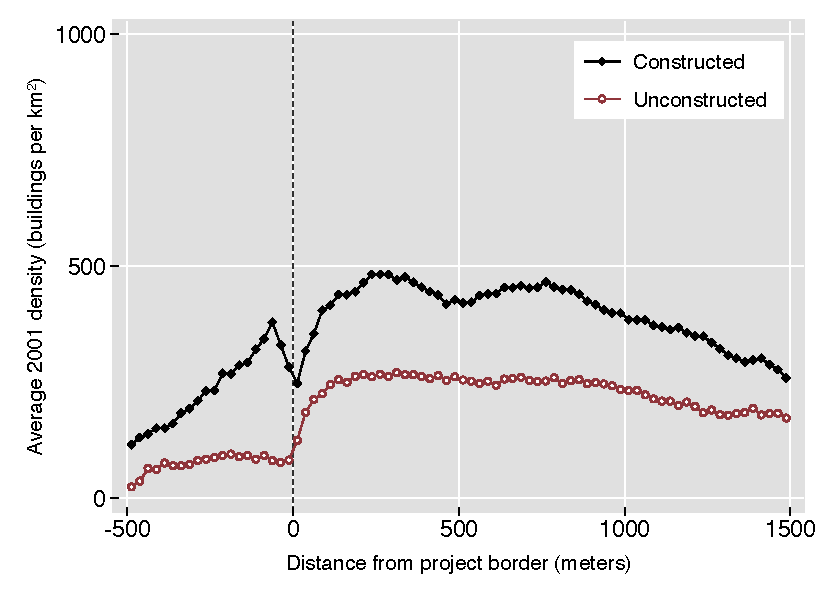
\includegraphics[width=\textwidth,trim={0.3cm .3cm 0.1cm 0cm}, clip=true]{figures/bblu_for_pre_means_4_spk.pdf}

%         \end{subfigure}
%         \hfill
%         \begin{subfigure}[b]{0.48\textwidth}  
%                     \caption[]%
%             {{\footnotesize \textbf{All Projects} pre-period informal  raw data}}      
%             \label{fig:preinf}
%             \centering 
%             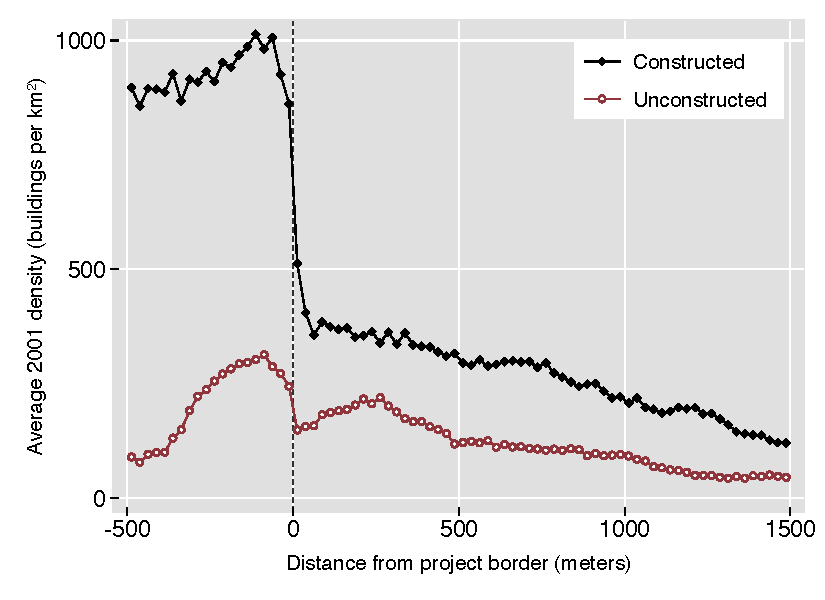
\includegraphics[width=\textwidth,trim={0.3cm .3cm 0.1cm 0cm}, clip=true]{figures/bblu_inf_pre_means_4_spk.pdf}

%         \end{subfigure}
%         \begin{subfigure}[b]{0.48\textwidth}
%                     \caption[Network2]%
%             {{\footnotesize \textbf{Greenfield} pre-period formal  raw data}}    
%             \label{fig:prefor}
%             \centering
%             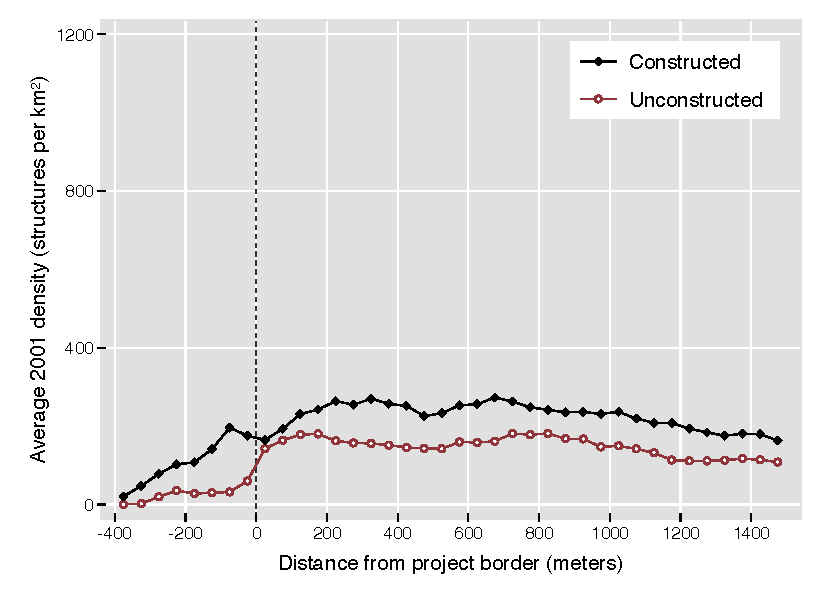
\includegraphics[width=\textwidth,trim={0.3cm .3cm 0.1cm 0cm}, clip=true]{figures/bblu_for_pre_means_4_1_spk.pdf}

%         \end{subfigure}
%         \hfill
%         \begin{subfigure}[b]{0.48\textwidth}  
%                     \caption[]%
%             {{\footnotesize \textbf{Greenfield} pre-period informal  raw data}}     
%             \label{fig:preinf}
%             \centering 
%             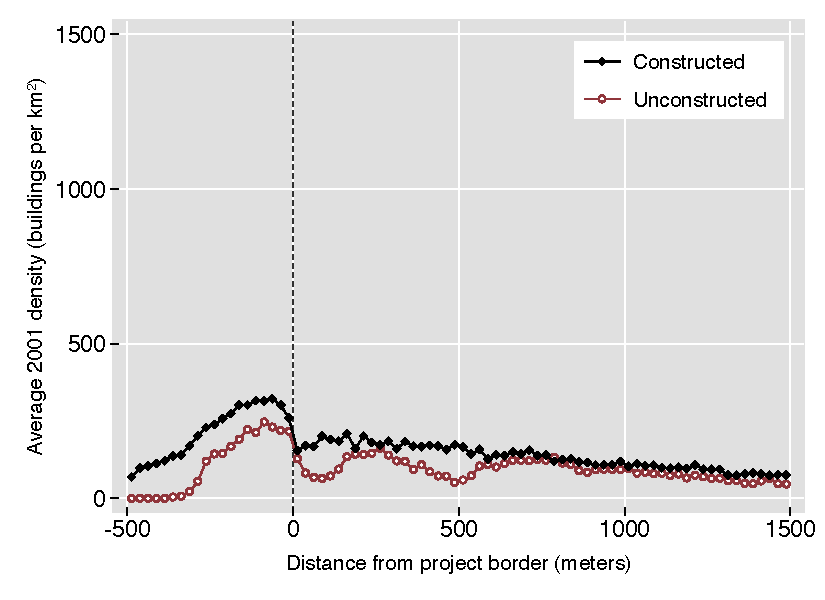
\includegraphics[width=\textwidth,trim={0.3cm .3cm 0.1cm 0cm}, clip=true]{figures/bblu_inf_pre_means_4_1_spk.pdf}

%         \end{subfigure}
%         \begin{subfigure}[b]{0.48\textwidth}
%                     \caption[Network2]%
%             {{\footnotesize \textbf{In-Situ} pre-period formal  raw data}}   
%             \label{fig:prefor}
%             \centering
%             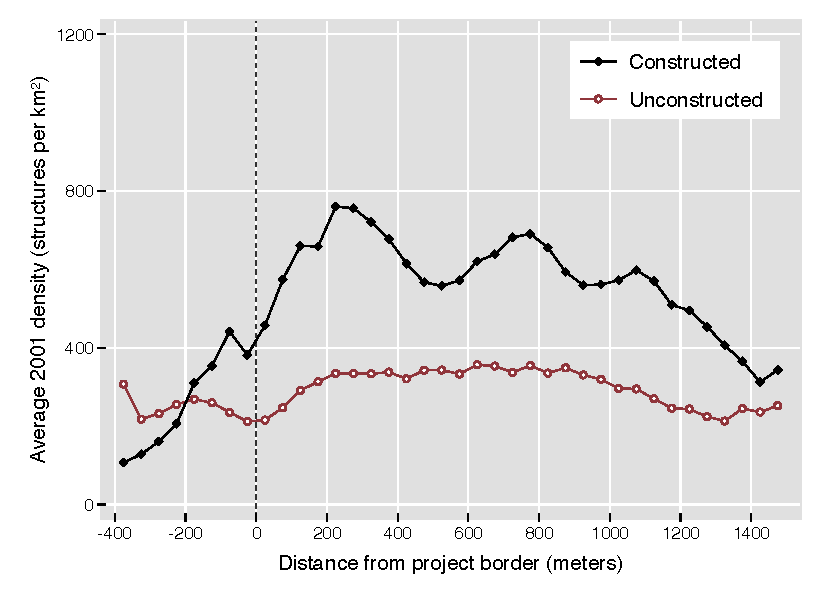
\includegraphics[width=\textwidth,trim={0.3cm .3cm 0.1cm 0cm}, clip=true]{figures/bblu_for_pre_means_4_2_spk.pdf}

%         \end{subfigure}
%         \hfill
%         \begin{subfigure}[b]{0.48\textwidth}  
%                     \caption[]%
%             {{\footnotesize \textbf{In-Situ} pre-period informal  raw data}}     
%             \label{fig:preinf}
%             \centering 
%             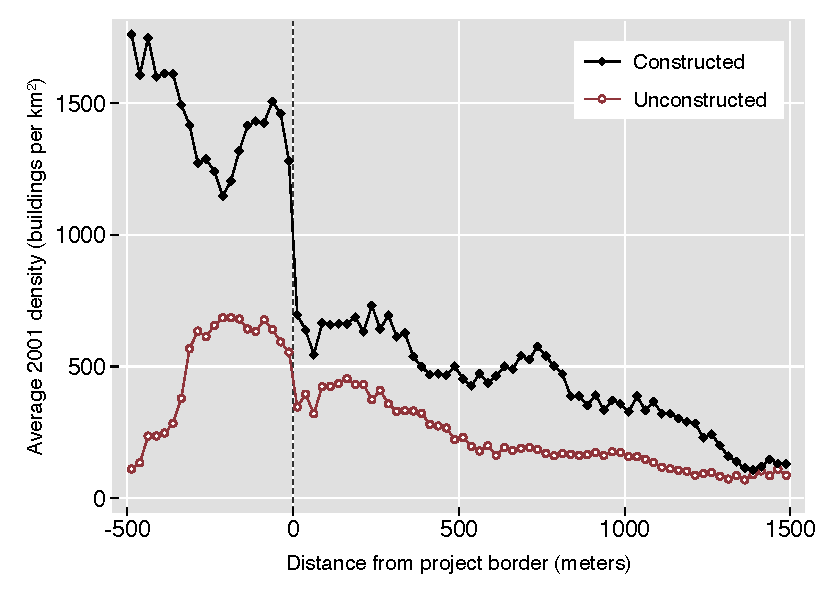
\includegraphics[width=\textwidth,trim={0.3cm .3cm 0.1cm 0cm}, clip=true]{figures/bblu_inf_pre_means_4_2_spk.pdf}

%         \end{subfigure}
%         \begin{subfigure}[b]{0.48\textwidth}
%                     \caption[Network2]%
%             {{\footnotesize \textbf{Other} pre-period formal  raw data}}   
%             \label{fig:prefor}
%             \centering
%             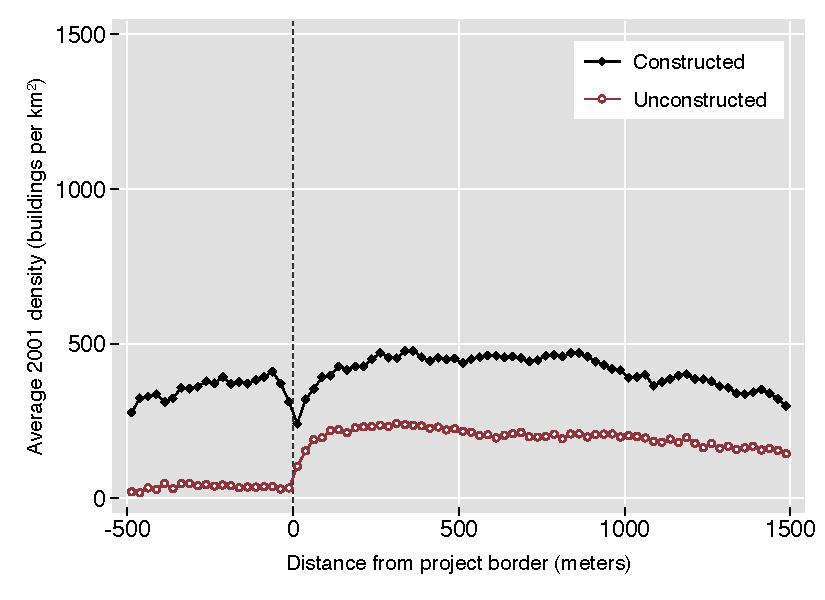
\includegraphics[width=\textwidth,trim={0.3cm .3cm 0.1cm 0cm}, clip=true]{figures/bblu_for_pre_means_4_3_spk.pdf}

%         \end{subfigure}
%         \hfill
%         \begin{subfigure}[b]{0.48\textwidth}  
%                     \caption[]%
%             {{\footnotesize \textbf{Other} pre-period informal  raw data}}      
%             \label{fig:preinf}
%             \centering 
%             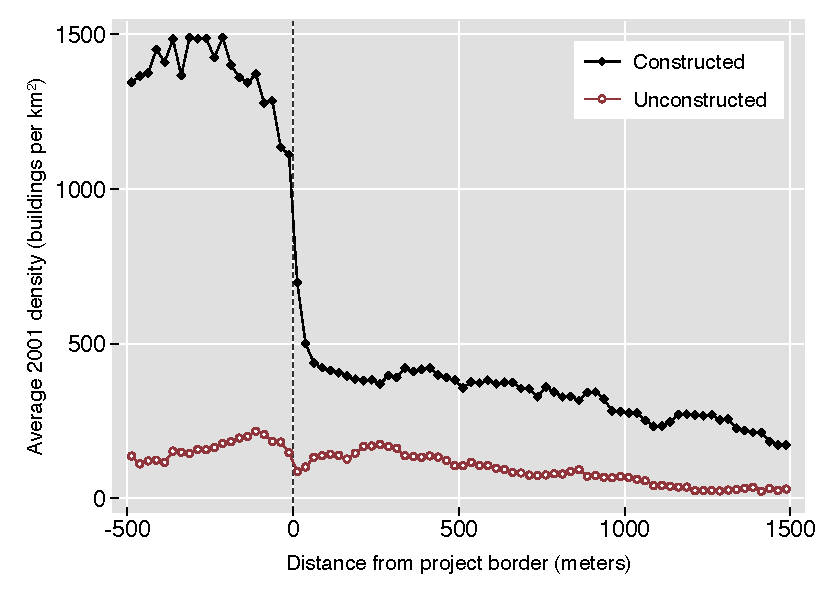
\includegraphics[width=\textwidth,trim={0.3cm .3cm 0.1cm 0cm}, clip=true]{figures/bblu_inf_pre_means_4_3_spk.pdf}

%         \end{subfigure}
% \end{figure*}








% \begin{figure*}
%         \centering
%    %     \caption[ Pre-Period Housing Densities in Constructed and Unconstructed Projects Areas ]
%   %      {\small Pre-Period Densities} 
%         %\vspace{2mm}
%         \begin{subfigure}[b]{0.48\textwidth}
%             \caption[Network2]%
%             {{\footnotesize \textbf{All Projects} changes formal raw data}}    
%             \label{fig:prefor}
%             \centering
%             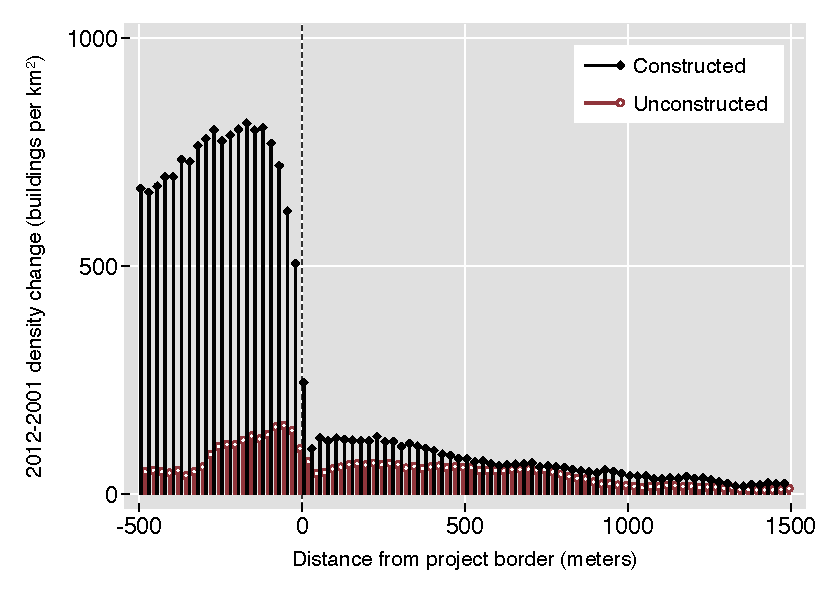
\includegraphics[width=\textwidth,trim={0.3cm .3cm 0.1cm 0cm}, clip=true]{figures/bblu_for_rawchanges_4_spk.pdf}

%         \end{subfigure}
%         \hfill
%         \begin{subfigure}[b]{0.48\textwidth}  
%                     \caption[]%
%             {{\footnotesize \textbf{All Projects} changes informal  raw data}}      
%             \label{fig:preinf}
%             \centering 
%             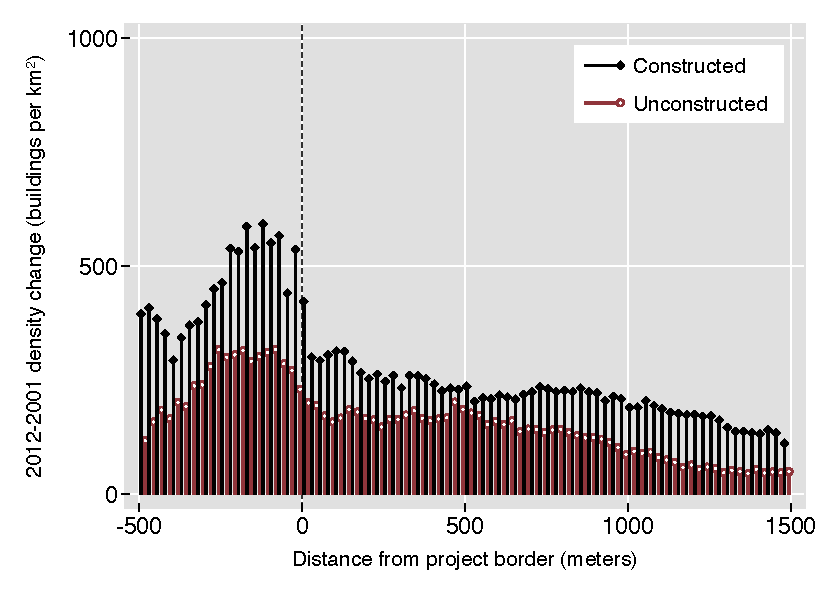
\includegraphics[width=\textwidth,trim={0.3cm .3cm 0.1cm 0cm}, clip=true]{figures/bblu_inf_rawchanges_4_spk.pdf}

%         \end{subfigure}
%         \begin{subfigure}[b]{0.48\textwidth}
%                     \caption[Network2]%
%             {{\footnotesize \textbf{Greenfield} changes formal  raw data}}    
%             \label{fig:prefor}
%             \centering
%             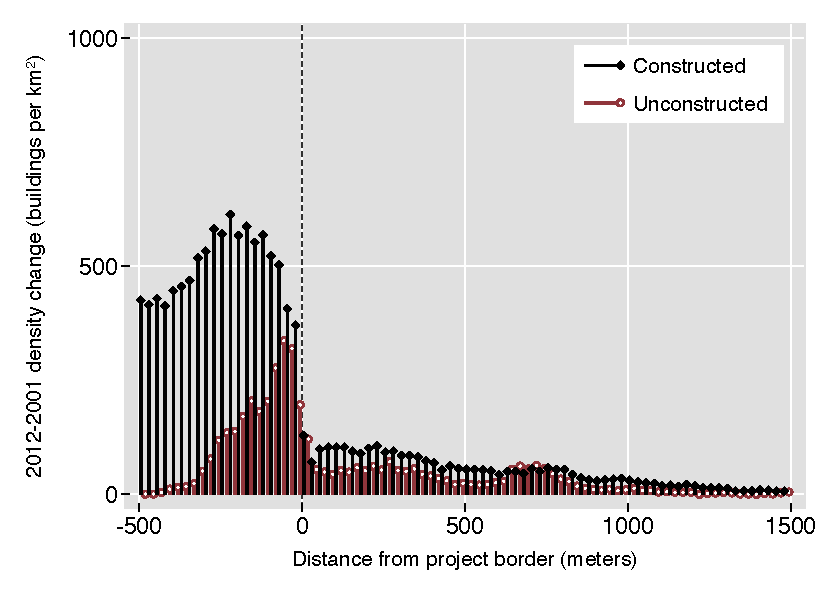
\includegraphics[width=\textwidth,trim={0.3cm .3cm 0.1cm 0cm}, clip=true]{figures/bblu_for_rawchanges_4_1_spk.pdf}

%         \end{subfigure}
%         \hfill
%         \begin{subfigure}[b]{0.48\textwidth}  
%                     \caption[]%
%             {{\footnotesize \textbf{Greenfield} changes informal raw data }}     
%             \label{fig:preinf}
%             \centering 
%             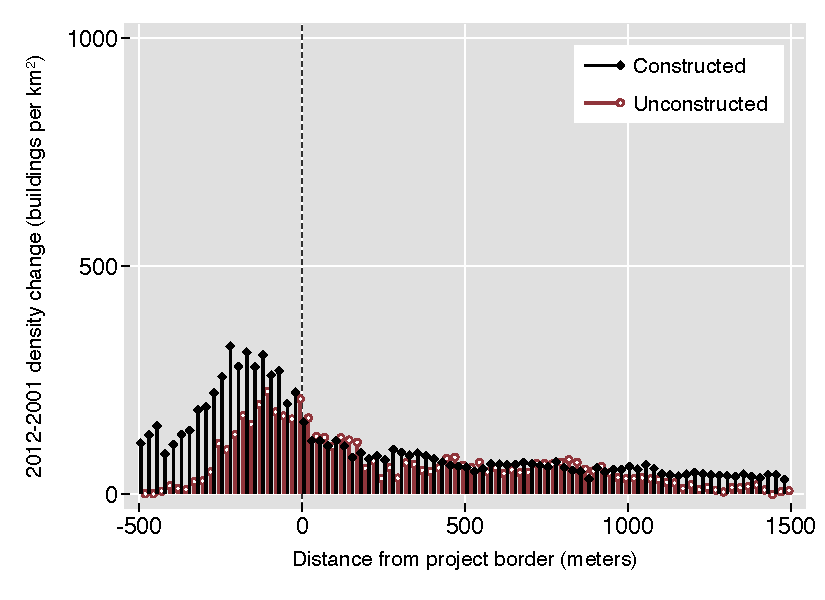
\includegraphics[width=\textwidth,trim={0.3cm .3cm 0.1cm 0cm}, clip=true]{figures/bblu_inf_rawchanges_4_1_spk.pdf}

%         \end{subfigure}
%         \begin{subfigure}[b]{0.48\textwidth}
%                     \caption[Network2]%
%             {{\footnotesize \textbf{In-Situ} changes formal raw data }}   
%             \label{fig:prefor}
%             \centering
%             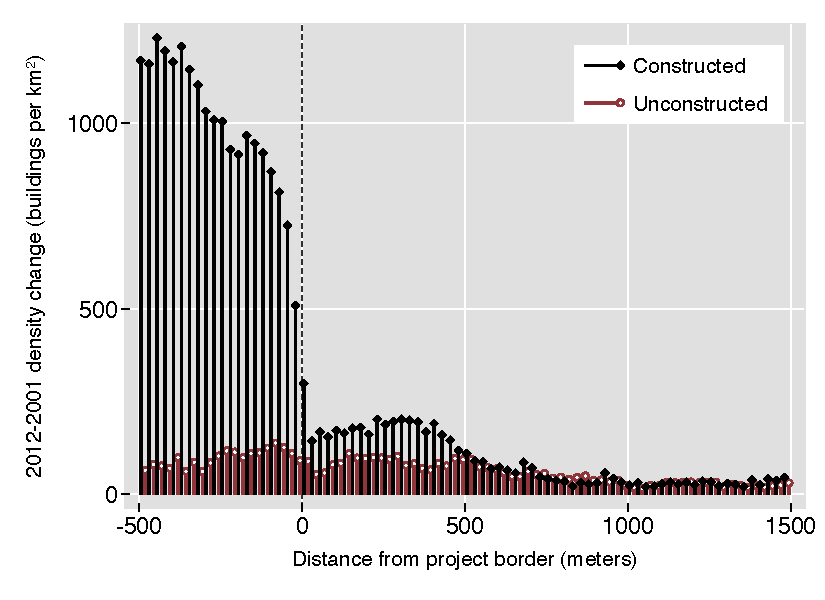
\includegraphics[width=\textwidth,trim={0.3cm .3cm 0.1cm 0cm}, clip=true]{figures/bblu_for_rawchanges_4_2_spk.pdf}

%         \end{subfigure}
%         \hfill
%         \begin{subfigure}[b]{0.48\textwidth}  
%                     \caption[]%
%             {{\footnotesize \textbf{In-Situ} changes informal raw data }}     
%             \label{fig:preinf}
%             \centering 
%             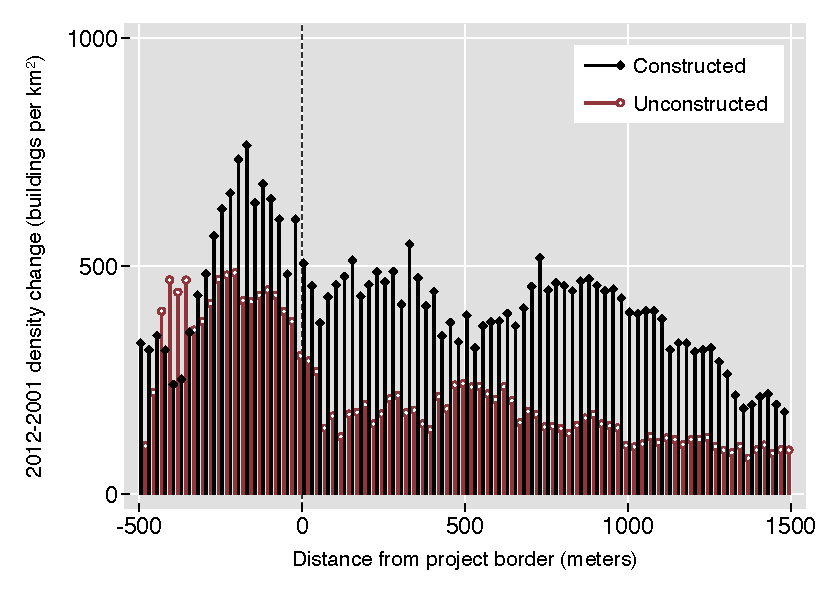
\includegraphics[width=\textwidth,trim={0.3cm .3cm 0.1cm 0cm}, clip=true]{figures/bblu_inf_rawchanges_4_2_spk.pdf}

%         \end{subfigure}
%         \begin{subfigure}[b]{0.48\textwidth}
%                     \caption[Network2]%
%             {{\footnotesize \textbf{Other} changes formal raw data}}   
%             \label{fig:prefor}
%             \centering
%             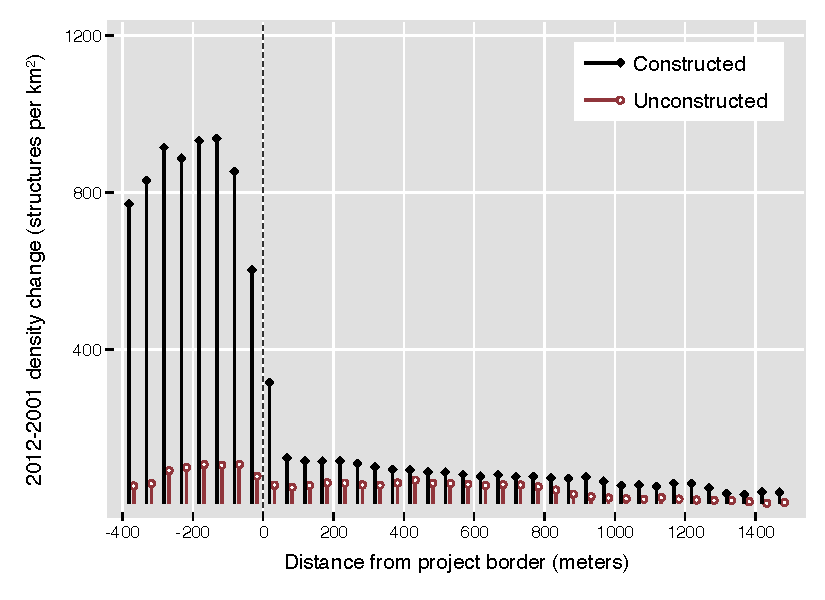
\includegraphics[width=\textwidth,trim={0.3cm .3cm 0.1cm 0cm}, clip=true]{figures/bblu_for_rawchanges_4_3_spk.pdf}

%         \end{subfigure}
%         \hfill
%         \begin{subfigure}[b]{0.48\textwidth} 
%                     \caption[]%
%             {{\footnotesize \textbf{Other} changes informal  raw data}}      
%             \label{fig:preinf} 
%             \centering 
%             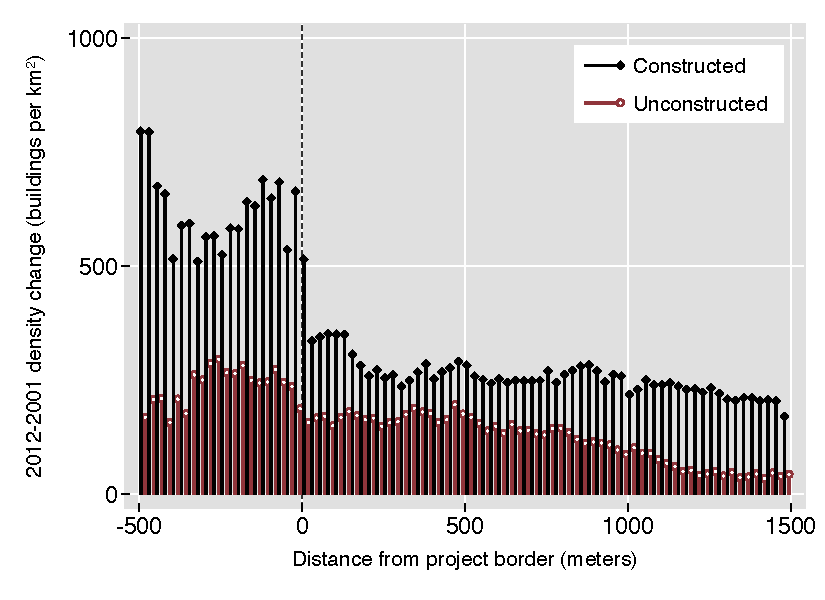
\includegraphics[width=\textwidth,trim={0.3cm .3cm 0.1cm 0cm}, clip=true]{figures/bblu_inf_rawchanges_4_3_spk.pdf}

%         \end{subfigure}
% \end{figure*}







\begin{table}
\caption{Building Density}
\begin{tabular}{lDDDDD}
\toprule
 & \small (1) & \small (2)  & \small (3) & \small (4) & \small (5) \\
 & Total & Formal  & Informal & Informal Bkyd. & Informal Non-Bkyd. \\ \midrule
\textbf{All Projects} \\inside project      &     430.447\textsuperscript{a}&     429.544\textsuperscript{a}&       0.904                   &     236.689\textsuperscript{a}&    -235.785\textsuperscript{a}\\
                    &   (142.814)                   &    (71.077)                   &   (103.801)                   &    (90.759)                   &    (71.637)                   \\[0.5em]
0-250m outside project &       1.389                   &      -3.240                   &       4.629                   &     -34.421                   &      39.050                   \\
                    &    (51.390)                   &    (21.950)                   &    (43.465)                   &    (36.896)                   &    (28.676)                   \\[0.5em]
250-750m outside project &     -61.379\textsuperscript{c}&     -17.677                   &     -43.702\textsuperscript{c}&     -42.755\textsuperscript{c}&      -0.948                   \\
                    &    (31.211)                   &    (12.747)                   &    (25.840)                   &    (22.313)                   &    (13.357)                   \\[0.5em]
R$^2$               &       0.442                   &       0.409                   &       0.405                   &       0.387                   &       0.346                   \\

\midrule
\textbf{Greenfield} \\   inside project      &     281.275                   &     217.960\textsuperscript{c}&      63.316                   &      91.741                   &     -28.425                   \\
                    &   (178.293)                   &   (112.664)                   &    (83.999)                   &    (80.736)                   &    (39.121)                   \\[0.01em]
0-250m outside project &     -31.114                   &     -22.847                   &      -8.267                   &     -43.751\textsuperscript{c}&      35.484                   \\
                    &    (48.971)                   &    (22.449)                   &    (35.611)                   &    (26.021)                   &    (29.653)                   \\[0.01em]
250-750m outside project &     -28.569                   &     -23.676                   &      -4.893                   &     -22.668\textsuperscript{b}&      17.775                   \\
                    &    (31.415)                   &    (16.703)                   &    (21.303)                   &    (10.394)                   &    (17.022)                   \\[0.8em] 
\textbf{In-Situ Upgrading} \\   inside project      &     234.312                   &     586.820\textsuperscript{a}&    -352.508                   &      28.093                   &    -380.601                   \\
                    &   (630.559)                   &   (164.487)                   &   (519.667)                   &   (439.428)                   &   (321.938)                   \\[0.01em]
0-250m outside project &      87.924                   &      67.953                   &      19.971                   &     -96.120                   &     116.091                   \\
                    &   (252.467)                   &    (92.486)                   &   (204.788)                   &   (190.681)                   &   (120.228)                   \\[0.01em]
250-750m outside project &     -22.414                   &      23.163                   &     -45.577                   &    -110.145                   &      64.569                   \\
                    &    (98.021)                   &    (35.792)                   &    (89.949)                   &    (74.795)                   &    (56.389)                   \\[0.8em]
\textbf{Other} \\   inside project      &     684.981\textsuperscript{a}&     596.824\textsuperscript{a}&      88.157                   &     449.974\textsuperscript{a}&    -361.817\textsuperscript{a}\\
                    &   (142.227)                   &    (72.363)                   &   (109.416)                   &   (107.543)                   &    (87.797)                   \\[0.01em]
0-250m outside project &     -15.843                   &       9.149                   &     -24.991                   &     -35.586                   &      10.595                   \\
                    &    (72.873)                   &    (27.986)                   &    (64.787)                   &    (51.479)                   &    (37.709)                   \\[0.01em]
250-750m outside project &    -103.662\textsuperscript{b}&     -19.442                   &     -84.220\textsuperscript{c}&     -49.206                   &     -35.015\textsuperscript{b}\\
                    &    (52.394)                   &    (18.745)                   &    (45.002)                   &    (42.005)                   &    (15.237)                   \\[0.8em]
Mean Outcome 2001   &      526.22                   &      261.56                   &      264.66                   &       96.43                   &      168.23                   \\
Mean Outcome 2011   &      838.62                   &      385.14                   &      453.48                   &      286.79                   &      166.69                   \\
R$^2$               &       0.443                   &       0.411                   &       0.406                   &       0.388                   &       0.347                   \\
N                   &   1,705,534                   &   1,705,534                   &   1,705,534                   &   1,705,534                   &   1,705,534                   \\

\bottomrule
\end{tabular}
\end{table}





\begin{table}[h!] 
\caption{Effect of Housing Projects on Socio-demographics}
\label{table:sorting}
\small
\centering
%\caption{Census Composition Estimates }
\vspace{-2mm}
\begin{tabular}{lDDDDD}
\toprule
& \small (1) & \small (2) & \small (3) & \small (4)& \small (5)\\
& \small Age & \small P.O.B. not Gauteng & \small Unemployed & \small Years of Education & \small Monthly Income \\ \midrule 
\textbf{All Projects} \\inside project      &       0.022                   &      -0.003                   &      -0.049\textsuperscript{b}&       0.224                   &     982.919\textsuperscript{c}\\
                    &     (0.408)                   &     (0.024)                   &     (0.022)                   &     (0.175)                   &   (582.996)                   \\[0.5em]
0-250m outside project &       0.318                   &      -0.015                   &      -0.031                   &       0.191                   &     453.044                   \\
                    &     (0.333)                   &     (0.018)                   &     (0.020)                   &     (0.137)                   &   (435.851)                   \\[0.5em]
250-750m outside project &       0.263                   &      -0.009                   &      -0.013                   &       0.043                   &     379.031                   \\
                    &     (0.259)                   &     (0.013)                   &     (0.016)                   &     (0.097)                   &   (408.310)                   \\[0.5em]
R$^2$               &       0.703                   &       0.771                   &       0.529                   &       0.692                   &       0.667                   \\

\midrule
\textbf{Greenfield} \\   inside project      &      -0.171                   &      -0.025                   &       0.008                   &       0.713\textsuperscript{b}&    1449.307                   \\
                    &     (0.688)                   &     (0.064)                   &     (0.048)                   &     (0.358)                   &  (1053.398)                   \\[0.01em]
0-250m outside project &       0.148                   &       0.016                   &       0.011                   &       0.216                   &     801.189                   \\
                    &     (0.750)                   &     (0.031)                   &     (0.049)                   &     (0.263)                   &   (710.706)                   \\[0.01em]
250-750m outside project &      -0.041                   &      -0.012                   &      -0.010                   &       0.347\textsuperscript{c}&     402.018                   \\
                    &     (0.749)                   &     (0.019)                   &     (0.041)                   &     (0.185)                   &   (516.752)                   \\[0.8em] 
\textbf{In-Situ Upgrading} \\   inside project      &       0.946                   &       0.053                   &      -0.073\textsuperscript{a}&      -0.084                   &     303.967                   \\
                    &     (0.642)                   &     (0.039)                   &     (0.028)                   &     (0.363)                   &  (1015.783)                   \\[0.01em]
0-250m outside project &       0.395                   &      -0.017                   &      -0.040                   &       0.072                   &     321.702                   \\
                    &     (0.392)                   &     (0.029)                   &     (0.035)                   &     (0.297)                   &   (917.230)                   \\[0.01em]
250-750m outside project &       0.370                   &      -0.020                   &      -0.033                   &      -0.147                   &     329.693                   \\
                    &     (0.308)                   &     (0.025)                   &     (0.022)                   &     (0.184)                   &  (1000.752)                   \\[0.8em]
\textbf{Other} \\   inside project      &      -0.058                   &      -0.022                   &      -0.050                   &       0.185                   &    1153.426                   \\
                    &     (0.516)                   &     (0.034)                   &     (0.031)                   &     (0.218)                   &   (853.396)                   \\[0.01em]
0-250m outside project &       0.476                   &      -0.014                   &      -0.035                   &       0.145                   &     233.980                   \\
                    &     (0.470)                   &     (0.027)                   &     (0.026)                   &     (0.162)                   &   (662.115)                   \\[0.01em]
250-750m outside project &       0.460                   &      -0.001                   &      -0.009                   &      -0.020                   &     358.892                   \\
                    &     (0.332)                   &     (0.020)                   &     (0.022)                   &     (0.135)                   &   (565.751)                   \\[0.8em]
Mean Outcome 2001   &       27.30                   &        0.37                   &        0.47                   &        8.27                   &    2,477.01                   \\
Mean Outcome 2011   &       28.30                   &        0.43                   &        0.33                   &        9.68                   &    4,486.48                   \\
R$^2$               &       0.705                   &       0.774                   &       0.530                   &       0.695                   &       0.670                   \\
N                   &      12,734                   &      12,727                   &      12,724                   &      12,728                   &      12,724                   \\

\bottomrule
\multicolumn{6}{l}{\footnotesize Standard errors clustered at the project level in parenthesis. \textsuperscript{c} p$<$0.10, \textsuperscript{b} p$<$0.05, \textsuperscript{a} p$<$0.01  }\\
\multicolumn{6}{l}{\footnotesize P.O.B. means ``place of birth.''  Monthly income is in Rands.}
\end{tabular}
\end{table}








\begin{landscape}
{\footnotesize

\begin{table}[]
\small
\centering
\caption{Census Household-level Estimates }\label{table:censusestimates}
\vspace{-2mm}
\resizebox{.9\linewidth}{!}{
\begin{tabular}{lDDDDDDDD}
\toprule
 & \small (1) & \small (2)  & \small (3) & \small (4) & \small (5)  & \small (6)  & \small (7) & (8)\\
 & \small Flush Toilet & \small Water Indoors  & \small Electricity Cooking & \small Electricity Heating & \small Electricity Lighting  & \small Number of Rooms  & \small Household Size & Population Density\\ \midrule 
\textbf{All Projects} \\inside project      &       0.069                   &       0.178\textsuperscript{a}&       0.110\textsuperscript{c}&       0.085                   &       0.063                   &       0.178                   &       0.053                   &   -1400.725                   \\
                    &     (0.056)                   &     (0.055)                   &     (0.062)                   &     (0.061)                   &     (0.068)                   &     (0.212)                   &     (0.090)                   &  (1181.130)                   \\[0.5em]
0-250m outside project &      -0.005                   &       0.105\textsuperscript{b}&      -0.022                   &      -0.026                   &      -0.032                   &       0.035                   &      -0.057                   &   -1308.129                   \\
                    &     (0.038)                   &     (0.046)                   &     (0.040)                   &     (0.039)                   &     (0.042)                   &     (0.154)                   &     (0.071)                   &  (1343.938)                   \\[0.5em]
250-750m outside project &      -0.026                   &       0.037                   &      -0.026                   &      -0.023                   &      -0.035                   &      -0.066                   &      -0.038                   &   -1366.876                   \\
                    &     (0.025)                   &     (0.030)                   &     (0.024)                   &     (0.022)                   &     (0.024)                   &     (0.108)                   &     (0.050)                   &  (1317.878)                   \\[0.5em]
R$^2$               &       0.616                   &       0.594                   &       0.669                   &       0.634                   &       0.639                   &       0.676                   &       0.692                   &       0.607                   \\

\midrule
\textbf{Greenfield} \\   inside project      &       0.163                   &       0.185                   &       0.218                   &       0.070                   &       0.172                   &       0.681\textsuperscript{c}&       0.045                   &     242.916                   \\
                    &     (0.144)                   &     (0.145)                   &     (0.133)                   &     (0.148)                   &     (0.132)                   &     (0.377)                   &     (0.204)                   &  (1754.516)                   \\[0.01em]
0-250m outside project &       0.059                   &       0.166\textsuperscript{c}&       0.032                   &      -0.011                   &      -0.015                   &       0.309                   &       0.177                   &   -2012.385                   \\
                    &     (0.076)                   &     (0.093)                   &     (0.058)                   &     (0.063)                   &     (0.068)                   &     (0.280)                   &     (0.158)                   &  (1492.218)                   \\[0.01em]
250-750m outside project &       0.018                   &       0.069                   &       0.027                   &       0.003                   &       0.005                   &      -0.035                   &       0.069                   &   -3889.888\textsuperscript{c}\\
                    &     (0.054)                   &     (0.066)                   &     (0.046)                   &     (0.050)                   &     (0.045)                   &     (0.174)                   &     (0.076)                   &  (2024.715)                   \\[0.8em] 
\textbf{In-Situ Upgrading} \\   inside project      &       0.020                   &       0.113                   &      -0.012                   &       0.048                   &      -0.113                   &      -0.133                   &      -0.068                   &   -2556.914                   \\
                    &     (0.113)                   &     (0.096)                   &     (0.125)                   &     (0.107)                   &     (0.138)                   &     (0.335)                   &     (0.147)                   &  (1913.995)                   \\[0.01em]
0-250m outside project &       0.038                   &       0.055                   &      -0.060                   &      -0.063                   &      -0.066                   &      -0.198                   &      -0.069                   &   -1977.568                   \\
                    &     (0.086)                   &     (0.085)                   &     (0.084)                   &     (0.080)                   &     (0.089)                   &     (0.249)                   &     (0.131)                   &  (2197.468)                   \\[0.01em]
250-750m outside project &      -0.019                   &       0.052                   &      -0.030                   &      -0.012                   &      -0.032                   &      -0.144                   &      -0.013                   &      96.675                   \\
                    &     (0.048)                   &     (0.058)                   &     (0.046)                   &     (0.052)                   &     (0.049)                   &     (0.195)                   &     (0.099)                   &  (1350.061)                   \\[0.8em]
\textbf{Other} \\   inside project      &       0.043                   &       0.188\textsuperscript{a}&       0.118                   &       0.086                   &       0.112                   &       0.178                   &       0.109                   &    -693.674                   \\
                    &     (0.077)                   &     (0.070)                   &     (0.086)                   &     (0.088)                   &     (0.091)                   &     (0.303)                   &     (0.118)                   &  (1243.780)                   \\[0.01em]
0-250m outside project &      -0.080                   &       0.099                   &      -0.055                   &      -0.034                   &      -0.054                   &       0.025                   &      -0.149\textsuperscript{c}&    -504.966                   \\
                    &     (0.050)                   &     (0.062)                   &     (0.053)                   &     (0.053)                   &     (0.056)                   &     (0.212)                   &     (0.084)                   &  (1389.797)                   \\[0.01em]
250-750m outside project &      -0.055                   &       0.018                   &      -0.044                   &      -0.034                   &      -0.049                   &      -0.020                   &      -0.105\textsuperscript{c}&    -879.813                   \\
                    &     (0.035)                   &     (0.040)                   &     (0.033)                   &     (0.030)                   &     (0.033)                   &     (0.158)                   &     (0.063)                   &   (948.344)                   \\[0.8em]
Mean Outcome 2001   &        0.79                   &        0.35                   &        0.66                   &        0.62                   &        0.77                   &        3.30                   &        3.51                   &    8,566.83                   \\
Mean Outcome 2011   &        0.83                   &        0.54                   &        0.81                   &        0.72                   &        0.82                   &        3.56                   &        3.18                   &    9,823.82                   \\
R$^2$               &       0.627                   &       0.603                   &       0.676                   &       0.640                   &       0.646                   &       0.681                   &       0.694                   &       0.609                   \\
N                   &      12,732                   &      12,732                   &      12,732                   &      12,732                   &      12,732                   &      12,709                   &      12,730                   &      12,734                   \\

\bottomrule
\multicolumn{9}{l}{\footnotesize All regressions include 3km grid Fixed-Effects. Standard errors clustered at the project level in parenthesis. \textsuperscript{c} p$<$0.10,\textsuperscript{b} p$<$0.05,\textsuperscript{a} p$<$0.01 }
\end{tabular}
}
\end{table}

}
\end{landscape}




\begin{table}
\small
\centering
\caption{Triple Difference Estimates on Log-Prices}\label{table:priceDDD_het}
\vspace{-2mm}
\begin{tabular}{lCC}
\toprule
 & \small (1) & \small (2)  \\ \midrule 
 \textbf{All Projects} \\
 inside project      &      -0.138                   &      -0.124                   \\
                    &     (0.271)                   &     (0.266)                   \\[0.55em]
0-250m outside project &       0.016                   &       0.022                   \\
                    &     (0.075)                   &     (0.074)                   \\[0.5em]
250-750m outside project &       0.091                   &       0.093                   \\
                    &     (0.057)                   &     (0.058)                   \\[0.5em]
Lot Size Controls   &                               &  \checkmark                   \\
r2                  &        0.52                   &        0.52                   \\
N                   &      67,751                   &      67,751                   \\

 \midrule
\textbf{Greenfield} \\   inside project      &       0.149                   &       0.021                   \\
                    &     (0.254)                   &     (0.254)                   \\[0.01em]
0-250m outside project &       0.209                   &       0.224                   \\
                    &     (0.222)                   &     (0.218)                   \\[0.01em]
250-750m outside project &       0.070                   &       0.074                   \\
                    &     (0.188)                   &     (0.191)                   \\[0.8em]
\textbf{In-Situ Upgrading} \\   inside project      &       0.133                   &       0.191                   \\
                    &     (0.349)                   &     (0.323)                   \\[0.01em]
0-250m outside project &      -0.120                   &      -0.120                   \\
                    &     (0.127)                   &     (0.126)                   \\[0.01em]
250-750m outside project &       0.089                   &       0.089                   \\
                    &     (0.109)                   &     (0.112)                   \\[0.8em]
\textbf{Other} \\   inside project      &      -0.270                   &      -0.230                   \\
                    &     (0.327)                   &     (0.319)                   \\[0.01em]
0-250m outside project &       0.097                   &       0.097                   \\
                    &     (0.100)                   &     (0.100)                   \\[0.01em]
250-750m outside project &       0.080                   &       0.078                   \\
                    &     (0.086)                   &     (0.086)                   \\[0.8em]
Lot Size Controls   &                               &  \checkmark                   \\
r2                  &        0.52                   &        0.52                   \\
N                   &      67,751                   &      67,751                   \\

\bottomrule
\multicolumn{3}{l}{\footnotesize Standard errors clustered at the project level in parenthesis.} \\
\multicolumn{3}{l}{ \textsuperscript{c} p$<$0.10,\textsuperscript{b} p$<$0.05,\textsuperscript{a} p$<$0.01 }
\end{tabular}
\end{table} 

% \begin{figure}
% 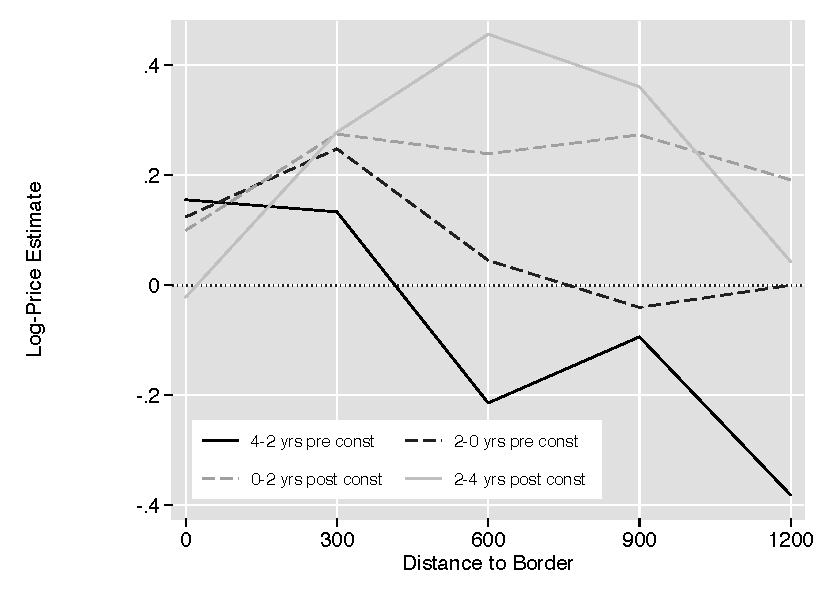
\includegraphics{figures/price_to_event_30.pdf}
% \end{figure}


\end{document}


